\documentclass[margin=5pt]{standalone}

\usepackage{tikz}
\usepackage{pgfplots}
\usepgfplotslibrary{patchplots}
\pgfplotsset{compat=1.3}

\begin{document}

    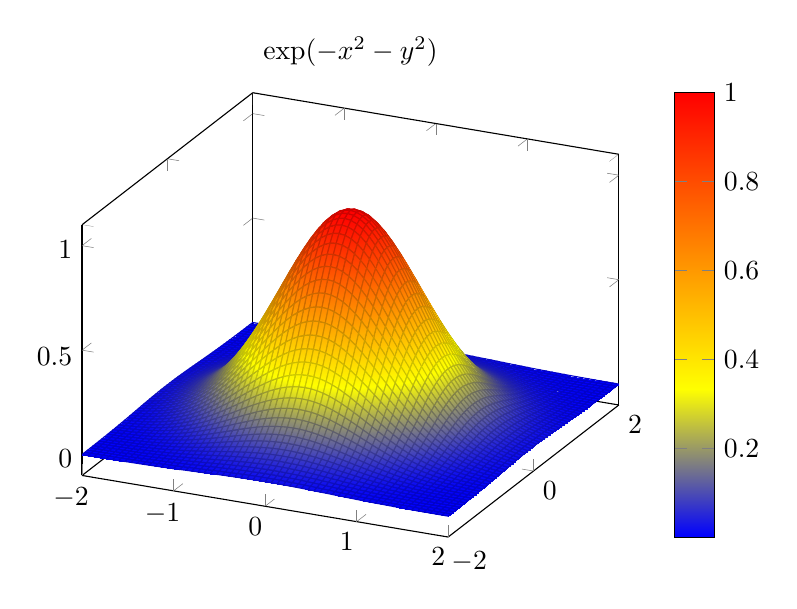
\begin{tikzpicture} 

        \begin{axis}[colorbar,title={$\exp(-x^2-y^2)$},]
        
            % Plot e^(-x^2-y^2) in 3D
            % No more than 61 samples, otherwise TeX will run out of memory
            % This plot takes a long running time
            \addplot3[surf,shader=faceted interp,samples=61,domain=-2:2] {exp(-x^2-y^2)};
        
        \end{axis}

    \end{tikzpicture}

\end{document}